%% config
\newcommand{\home}{../../latex/styles} % home directory - need for absolute paths with 

%% documentclass
\input{\home/documentclass_normal_oneside}

%% generell-styling
\include{\home/style_proggen}

%% meta-tags for pdf
\newcommand{\pdfauthor}{Matthias Günther}
\newcommand{\pdftitle}{git}
\newcommand{\pdfsubject}{Aufzeichnungen zur Fortbildung}
\newcommand{\pdfkeywords}{git, svn, SCM, SVN}
\newcommand{\motto}{Scala - just scale your large applications}
\newcommand{\tutor}{}
\newcommand{\disclaimer}{(Die Autoren übernehmen keine Garantie und Haftung 
für die Korrektheit des Skriptes. Das Skript ist unter den Namen von Matthias 
Günther veröffentlich.)}
\newcommand{\publisher}{Der Helex-Matze Verlag $\sum\limits_{i=1}^{n}i$}
\newcommand{\pdfemail}{matthias.guenther@wikimatze.de}
\newcommand{\correctiontext}{Kommentare/Korrekturen an}
\newcommand{\homepagetext}{Homepage}
\newcommand{\homepage}{wikimatze.de}
\newcommand{\coverdisclaimer}{Copyright Skript-Covers}
\newcommand{\covercopyright}{\textsc{Ubisoft} (\url{ubi.com})}

% label for programming-language


%% fancy-header
\input{\home/style_header_oneside}

%% setting the infos for the pdf
\input{\home/info_hypersetup}

%% environments
\input{\home/style_environments_normal}

%% cover
\input{\home/style_cover_german}

% label for programming-language
\input{\home/style_scala}
\begin{document}
\input{\home/style_starting_document_without_cover}


\section{Einführung}
\begin{itemize}
  \item \textbf{Kompilierung}: \texttt{scalac}\footnote{Resultat sind JVM Klassen-Datein, welche man in JARs packen kann, hierbei wird jedoch class, trait \oder object-Definition verlangt} bzw. \texttt{fsc}\footnote{schnellere Kompilierung}
  \item \textbf{Ausführung}:\footnote{Programm wird kompiliert \und danach gleich ausgeführt} \texttt{scala}
\end{itemize}


\subsection{Einfache Programme}
\begin{itemize}
  \item Hello Helex:
  
  \lstinputlisting[label=src:hello_helex.scala]{beispiele/hello_helex.scala}
  
  $\Rightarrow$ Datei muss wie das Objekt heißen, damit es ausgeführt werden
  kann
  \item Zahlen:
  
  \lstinputlisting[label=src:numbers.scala]{beispiele/numbers.scala}
  
  \item ein Programm, dass ein String in Int parsed und dabei alle Zahlen der Eingabe aufsummiert:
  
  \lstinputlisting[label=src:input_parsing.scala]{beispiele/input_parsing.scala}
  
  \begin{itemize}
    \item \itbf{Option}:
    \begin{itemize}
      \item \texttt{Option} ist Container, der Null (dann ists 
      \texttt{None}) \oder ein Element dann ists \texttt{Some(theElement)}
      enthält
      \item durch Option verhindert man \texttt{null} Pointer Exceptions
      
      $\Rightarrow$ gut wenn man Business-Logik schreibt und diesen Fall
      nicht in jeder Abfrage, sondern einfach am Ergebnistyp der Funktion
      festlegt\footnote{denke an Adminbill aus pictrs}
      \item Parsing des Strings: sollte eben keine zahl eingegeben
      werden, so wird keine Exception geworfen, sondern die Ausgabe
      einfach auf \texttt{None} gemappt
    \end{itemize}
    \item \itbf{sum}
    \begin{itemize}
      \item in der Methode \texttt{sum} definieren wir keinen return-Wert
      \item \texttt{in} Parameter ist vom Typ 
      \texttt{Seq}\footnote{\texttt{Seq} ist \textit{supertrait} von 
      \texttt{Array, List} \und andere \textit{Collections}}, was ein 
      ein \textit{trait}\footnote{denke Interface aus Java} ist
      \item \texttt{traits}\footnote{traits beheben das Diamanten-Prob. 
      der multiplen Vererbung, da eine Klasse beliebig viele traits haben} 
      können implementierte Methoden beinhalten \und sind am Besten mit 
      mixins aus Ruby zu vergleichen
      \item mit \texttt{flatMap} ruft die Methode \texttt{toInt}
      für jedes Element der Sequenz in \texttt{in} auf
      \item mit $s => toInt(s)$ definieren wir eine anonyme
      Funktion, die einen einzelnen Parameter $s$ nimmt \und diesen
      an die Funktion \texttt{toInt} weitergibt
      \item \texttt{foldLeft}\footnote{kann man gut verwenden, wenn man die 
      Werte einer Sequenz aufsummieren will} nimmt einen einzelnen Parameter als
      \textit{seed} \und und schreibt das Ergebnis der inneren
      Funktion an diesen \textit{seed} zurück. Dabei wird der 
      \textit{seed} solange weiter $\uparrow$, bis alle Elemente der 
      Sequenz durchlaufen wurden
    \end{itemize}
  \end{itemize}
\end{itemize}
\pagebreak


\section{Eigenschaften zur Sprache}
\begin{itemize}
  \item Wofü Scala geeingnet ist:\textit{language ideal for today’s scalable,
  distributed, component-based applications that support concurrency and
  distribution}
  \item \textbf{Merke}: \textit{Is a statically typed\footnote{der Typ 
  einer Variable ist für die gesamte Lebenszeit der Variable fest}, 
  mixed-paradigm, JVM language with a succinct, elegant, and flexible 
  syntax, a sophisticated type system, and idioms that promote 
  scalability from small, interpreted scripts to large, 
  sophisticated applications.}
  \item Programmiersprachen für Softwarekomponenten müssen \textbf{skalierbar}
  sein $\Rightarrow$ Konzentration bei Scala auf Abstraktion, Komposition
  und Dekomposition
  \item skalierbare Unterstützung für Komponenten kann nur erreicht werden,
  wenn OOP generalisiert und mit funktionalen Aspekten (FP) einer
  Programmiersprache vereinigt werden
  \item Scala arbeitet gut mit Java und C\# zusammen
  \item Typsystem von Scala hat folgende Vorteile:
  \begin{enumerate}
    \item Abstrakte Typdefinitonen und vom Pfad 
    abhängige Typen\footnote{\enquote{\textit{v}Obj calculus}} unterstützen
    \item modulare mixing Komposition
    \item \textit{views}\footnote{ermöglichen Komponenten-Adaption in 
    einem modularen Weg}
  \end{enumerate}
  \item Scala Klassen \und Objekte können von Java-Sachen erben \und Java-
  Interfaces implementieren $\Rightarrow$ man kann Scala-Code in einem 
  Java-Framework\footnote{wicket} verwenden
  \item \textbf{high-order functions}: sind Funktionen, die Funktionen als
  Argumente nehmen \oder Funktionen als Ergebnis zurückliefern \und diese
  werden von Scala unterstützt
  \item \textbf{scope} verschachtelte Funktionen können auf alle Parameter 
  \und lokalen Variablen innerhalb ihrer Umgebung zugreifen
  \item Funktionen-Def mit nur einer Zeile benötigen keine geschweiften Klammern
  \item \textbf{id: type}-Syntax wird von Scala verwendet 
  \item \textbf{unit} wird statt void in Scala verwendet
  \item Scala hat eine Darstellung on Javas \texttt{void}, nämlich 
  \texttt{Unit}\footnote{kann man explizit zurückgeben, wenn man einfach
  () beim Returnwert einer Funktion hinschreibt}
  \item alle Kontrollstrukturen von Java sind auch in 
  Scala\footnote{for-Schleifen wurde stark vereinfacht :)} vorhanden
  \item in Scala hat alles einen öffentlichen Zugriff, es sein denn
  es wird anders definiert
  \item \textbf{Klassen mit Argumenten}: Argumente dienen als
  Konstruktoren für die Klasse
  \item Scala-Objekt ist Instanz einer Klasse \und kann deswegen als
  Parameter von Methoden agieren kann
  \item Klassen, Objekte \und \itbf{traits}\footnote{um es in Java-Sprache
  auszudrücken sind \textit{traits} Interfaces mit einer Superklasse, die
  nicht-abstrakte Methoden beinhalten dürfen} können innere Klassen, Objekte
  \und traits haben, welche Zugriff auf \textit{private} Methoden,
  Variablen und so weiter haben
  \item die Import-Methode kann innerhalb von Blöcken verwendet werden
  $\Rightarrow$ können dadurch feingranular den scope festlegen
  \item Scala ist statisch typisiert
  \item \textbf{Nothing}: eine Methode mit diesen Rückgabewert, wird
  normalerweise niemals laufen
  \item \textbf{Any} ist die Mutter aller Klassen in Scala
  \item \textbf{AnyRef} bedeutet dasselbe wie Javas \texttt{Object},
  jedoch mit den Unterschied, dass mit == die inhaltliche Gleichheit von 
  Objekten gemeint ist - will man die Referenz von Objekten beurteilen,
  dann nimmt man lieber die Methode \texttt{eq}
  \item der return-Wert von Funktionen ist per default die letzte Zeile einer
  Methode\footnote{man kann aber auch explizit return angeben}
  \item \textbf{call-by name} kann man in Scala durch $=>$ für Funktionsaufrufe 
  anfordern:
  
  \lstinputlisting[label=src:call_by_name.scala]{beispiele/call_by_name.scala}
  
  $\Rightarrow$ es kommen verschiedene Zeiten heraus $\Rightarrow$ in
  \textit{delayed} wird bereits reingegangen bevor \textit{nano} 
  aufgerufen wird und somit wird \textit{nano} zweimal aufgerufen
  \item \texttt{[B $>:$ T]} heißt, dass \texttt{B} mindestens von derselben
  Klasse wie \texttt{T}
  \item \textbf{impliziten Konversion}: man fügt einer eigentlichen als 
  \texttt{final} deklarierten Klasse noch
  zusätzliche Methoden hinzu\footnote{einfach implicit vor Methodendef
  schreiben}
  \item Scala ist FP, d.h. in dem Sinne, dass jede Funktion einen Wert hat
  \item Scala ist statisch Typisiert \und das Typsystem unterstützt:
  \begin{itemize}
    \item \textbf{generische Klassen}
    \item \textbf{Varianz}-Annotationen
    \item obere \und untere Schranken für Typen
    \item \itbf{compound types}
    \item polymorphe Methoden
    \item Scala ist erweiterbar: man kann leicht neue Sprachkonstrukte
    zur Sprache ergänzen
  \end{itemize}
  \item Scala kompiliert in normalen Java Bytecode
  \item Scala arbeitet gut mit Java \und .NET an
  \item jede Java Klasse kann als eine normale Scala-Klasse verwendet werden
  $\Rightarrow$ deswegen sind alle Java-Bibos auch direkt in Scala verwendbar
  \item gewöhnlicher Java-Code ist kein valider Scala-Code, aber wenn der
  Java-Code einmal kompiliert wurde, dann kann er vom Scala-Code verwendet
  werden
  \item Scala läuft wie Java auf derselben JVM \und sie teilen sich deshalb
  den gleichen Garbage-Collector
  \begin{itemize}
    \item auf Java Bytecode kann Scala:
    \begin{itemize}
      \item Objekte instanziieren
      \item Methoden aufrufen
      \item exceptions werfen/abfangen
      \item Klassen erweitern
      \item Interfaces implementieren
    \end{itemize}    
    \item Java-Klassen als Mixins, wenn diese als Quellcode vorhanden
    sind
    \item Java \enquote{locking \und concurency model} wird unterstützt, wird
    aber normalerweise von Scala gerwapped
  \end{itemize}
  \item Imports sind wie in Java, nur mit mehr Features (denke ans
  Alias) \und imports können allen Stellen des Programms gemacht werden
  \item wenn Typen offensichtlich sind, dann muss man diese nicht angeben, kann
  aber zu bösen Fehlern führen
  \item Generics\footnote{statt Generics sagt man in Scala zu 
  dynamischen Datentypen von Funktionen \itbf{parameterized types}}:
  \begin{itemize}
    \item Klassen \und traits können generisch gemacht werden
    \item via \itbf{Typparameter} (Nonvariant, Covariant, Contravariant)
    \item obere \und untere Schranken
  \end{itemize}
  \item FP Eigenschaften: \textit{Higher-order functions}; 
  \textit{Function closure support}; Rekursion als \textit{flow control}; 
  \textit{pure Funktionen} $\Rightarrow$ keine 
  Seiteneffekte\footnote{viele Datenstrukturen sind immutable, mit 
  \texttt{val} sind immutable \und mit \texttt{var} sind mutable};
  \textit{Pattern Matching}
  \item immutable \texttt{val} müssen initialisiert werden!  
  \item Klassen können überall in einem Programm auftauchen: top-level,
  innerhalb von anderen Klassen (\textit{inner classes}), innerhalb von
  Codeblöcken (\textit{local classes}) \und innerhalb von Ausdrücken 
  (\textit{anonymous classes}) $\Rightarrow$ analog gilt das für Funktionen
  in Scala, nur das Funktionen nicht als Top-Level deklariert werden können
  \item Scala ist eine stark typisierte Sprache: \textit{class types},
  \textit{variant class type parameters}, \textit{virtual types}, 
  \textit{qualified class types},  \textit{compound types}\footnote{kann
  man festlegen, dass ein Wert eine Instanz von einer Liste von Klassen
  ist}, \textit{singleton types}\footnote{für Typen gibt es genau einen
  Wert}, \textit{explicit self types}\footnote{sind Annotationen, die den Typ 
  einer aktuellen Instanz einer Klasse festlegen}
  \item Scala unterstützt \itbf{Symbole} aus Ruby
  \item \texttt{null} gibts in Scala, aber ab in die Tonne damit \und 
  besser \texttt{Option} verwenden
  \item wenn man \textbf{final} vor Klassen \oder traits schreibt, dann
  verhindert man, dass davon Klassen abgeleitet werden können
  \item \textbf{super} ist analog zu this, aber es bindet an die Elternklasse
  \item \textbf{this} wie ein Objekt auf sich alleine zeigt
  \item das \$ verwendet Scala intern für irgendwas, also ebenso wie
  die keywords nicht als Variablennamen verwenden
  \item Scala-Konvention: Klammern bei Methodenaufrufen vermeiden, wenn
  diese keine Seiteneffekte verursachen
  \item \itbf{Generatoren}:
  
  \lstinputlisting[label=src:generators.scala]{beispiele/generators.scala}
  
  der \textit{left-arrow} Operator wird eben Generator genannt, der er die
  einzelnen Elemente aus der Collection generiert
\end{itemize}


\subsection{Paradigmen}
\ulbf{\kreis{1. } OOP-Paradigma}



\begin{itemize}
  \item alles ist ein Objekt
  \item Scala hat die typischen Mechanismen von OOP, aber ergänzt das ganze
  noch durch \textit{traits}, \textit{mixin composition}
  \item es gibt keine primitven Datentypen wie in Java, anstelle sind alle 
  numerischen Typen Objekte
  \item Scala unterstützt \textit{singleton object construct}
\end{itemize}


\ulbf{\kreis{2. }FP-Paradigma}


\begin{itemize}
  \item FP sind gut für Design-Probs wie \textit{concurrency}, da pure FP
  keine $\Delta$ Zustände erlaubt\footnote{um Synchronisation muss man
  sich nicht kümmern}
  \item in puren FP kommunizieren Programme durch den Autausch von
  nebenläufigen autonomen Prozessen $\Rightarrow$ Scala unterstützt dass
  durch seine \texttt{Actors Library}, aber es unterstützt auch
  veränderliche Elemente, wenn man das will
  \item Funktionen sind \itbf{first class}\footnote{d.h. sie können 
  an Variablen, an andere Funktionen usw. ähnlich wie Werte übergeben werden}
  \und Scala bietet \itbf{closures}\footnote{bezeichnet man 
  eine Programmfunktion, die beim Aufruf einen Teil ihres vorherigen
  Aufrufkontexts reproduziert, selbst wenn dieser Kontext außerhalb der 
  Funktion schon nicht mehr existiert $\Rightarrow$ sind ein mächtiges 
  Werkzeug zur Abstraktion} 
\end{itemize}


\ulbf{\kreis{3. } Skalierbarkeit}\footnote{es wurde designt, um von kleinen, interpretierten
Skripten zu großen, verteilten Anwendungen zu skalieren} wird durch folgende
Sachen gewährleistet:


\begin{enumerate}
  \item explizite \textit{self types}
  \item abstrakte \textit{type members} \und \textit{generics}
  \item verschachtelte Klassen
  \item \textit{mixin} Komposition durch Verwendung von \textit{traits}
\end{enumerate}


\ulbf{\kreis{4. }Performanz}


\begin{itemize}
  \item da Scala ja auf der JVM läuft, unterstützt auch die ganzen dafür
  entwickelten Optimierungsmethoden (Profilers, verteilter Cache, Clustering)
\end{itemize}


\subsection{Klassen}
\begin{itemize}
  \item werden in Packeten definiert \und spielen eine ähnliche Rolle wie
  in Java
  \item jedes Java-Packet ist auch eine Scala-Packet (vice versa)
  \item jede Klasse kann via \textit{mixin} von mehr als einer Klasse
  erben, denn per default kann nur von einer Klasse gererbt werden
  \item jede Java-Klasse wird als gewöhnliche Scala-Klasse angesehen \und 
  jedes Java-Interface kann als Scala-\textit{trait} angesehen werden
\end{itemize}


\subsubsection{Klassenhierarchie}
\begin{itemize}
  \item in Scala ist alles, bis auf eine Methode eine Instanz von
  einer Klasse $\Rightarrow$ alle Primitven aus Java (wie \uline{z.B.} int) 
  werden als Instanzen behandelt \und dies wird bei Kompilierung gemacht
  \item \texttt{Any} ist die Top-Klasse, es hat zwei Unterklassen:
  \texttt{AnyVal} \und \texttt{AnyRef}
  \item \texttt{AnyVal}  basiert auf \textit{value classes}, also
  \textbf{boolean, byte, short, char, int, long, float, double}
  \item wenn man sich an die Namenskonventionen hält, dann sind
  die Scala-Repräsentanten der Primitiven Datentypen der JVM:
  \begin{itemize}
    \item \texttt{Int}
    \item \texttt{Long}
    \item \texttt{Double}
    \item \texttt{Float}
    \item \texttt{Boolean}
    \item \texttt{Char}
    \item \texttt{Byte}
  \end{itemize} 
  
  alle Unterklassen von der Klasse \texttt{AnyVal}
\end{itemize}


\subsubsection{Klassenimport}
\begin{itemize}
  \item Syntax:
  
  \lstinputlisting[label=src:import.scala]{beispiele/import.scala}
  
  \item mehrere Klassen \oder Objekte können vom selben Paket importiert werden, 
  indem sie einfach in \textit{brackets} geschrieben werden
\end{itemize}


\subsection{Scala hat uniformes Objektmodel}
$\Rightarrow$ d.h. jeder Wert ist ein Objekt \und jede Operation ist ein
Methodenaufruf


\begin{itemize}
  \item Mutterklasse aller Scala-Klassen ist \texttt{Scala.Any}
  \item am untersten Ende der Scala-Typen steht \texttt{scala.Null}
  \und \texttt{scala-Nothing}
  \item \texttt{scala.Null} ist ein \textit{subtype} von allen Referenztypen
  
  $\Rightarrow$ einzige Instanz ist die \textbf{null} Referenz
  \item \texttt{scala.Nothing} ist \textit{subtypen} von jeden anderen Typen
  
  $\Rightarrow$ von diesen Typen existieren keine Instanzen
  \item Scala behandelt das auftauchen von Bezeichnern zwischen zwei
  ausdrücken als Methodenaufruf
  \item Scala erlaubt die Definition von parameterlosen Methoden \und jedesmal
  wird so eine Funktion aufgerufen, wenn dessen Name verwendet wird
  \item man kann auch abstrakte Klassenvariablen anlegen, ohne dass man den
  \textit{modifier} \textbf{abstract} davor schreiben muss
  \item In Scala folgen Konstruktor-Parameter den Klassennamen
  \lstinputlisting[label=src:klassen_constructor.scala]{beispiele/klassen_constructor.scala}
  \item Scala braucht den \textbf{override} \textit{modifier}, wenn konkrete
  Methoden einer geerbten Methode überschrieben werden sollen (sollte man eine
  Methode in einer Subklasse ohne den \textit{override} überschreiben, so meckert
  der Compiler, sollte man in einer Oberklasse die Parameteranzahl einer Funktion
  ändern, welche in einer geerbten Klasse noch mit der vorherigen Parameterzahl
  besteht, so macht der Compiler aus dieser eventuell gewollt überschriebenden
  Methode einfach ein überladen)
  \item der $=>$ Operator gibt an, dass aktuelle Argumente für diesen Parameter
  unausgewertet übergeben werden.
    
  die Argumente einer solchen Funktion werden jedesmal ausgewertet, wenn der
  formale Parameter erwähnt wird
  
    \lstinputlisting[label=src:unausgewertete_parameter_uebergabe.scala]{beispiele/unausgewertete_parameter_uebergabe.scala}

  \item für jede Variable \textbf{var} \textit{x: T} definiert Scala
  die folgenden \textit{setter} und \textit{getter} Methoden:
  
  \lstinputlisting[label=src:getter_setter.scala]{beispiele/getter_setter.scala}
  
  diese Methoden referenzieren und updaten die entsprechende Speicherzelle für
  die Variable, welche nicht direkt durch Scala-Programme beeinflussbar ist
  
  \item die Behandlung von Variablenzugriffen als Methodenaufrufen ermögicht
  es in Scala \textbf{properties} zu definieren. Im folgenden Beispiel wird
  die Eigenschaft \textit{degree} definiert, welche nur einen Wert entspricht,
  der größer \oder gleich -273 ist
  
  \lstinputlisting[label=src:properties.scala]{beispiele/properties.scala}
  
\end{itemize}


\subsection{Operationen sind Objekte}
$\Rightarrow$ kommt daher, dass Scala eine funktionale Sprache ist, d.h. 
jede Funktion hat einen Wert


\ulbf{Methoden sind funktionale Werte}


\begin{itemize}
  \item betrachten die folgende Funktion, welche überprüft, ob ein Array eine
  Element mit einer bestimmten Eigenschaft (Prädikat) hat:
  
  \lstinputlisting[label=src:array.scala]{beispiele/array.scala}
  
  \begin{itemize}
    \item der Elementtyp des Arrays ist beliebig, wird durch den Parameter [T]
    angegeben der exists-Methode\footnote{ist eben was generisches} angegeben 
    \item die zu testende Eigenschaft ist beliebig \und dies wird durch
    den Parameter $p$ der exists-Methode repräsentiert
    \item der Typ von \texttt{p} ist der \textit{Funktionstyp} $T => boolean$,
    welche als Werte alle Funktionen mit der Domäne $T$ und den Bereich von
    $boolean$ hat
    \item Funktionsparameter können wie normale Funktionen angewendet werden 
    (siehe im $p$ in while-Schleife)
    \item mithilfe der obigen Funktion können wir eine Funktion \texttt{forall}
  via Doppelnegation erstellen: Ein Prädikat gilt für alle Elemente eines Arrays,
  wenn es kein Argument gibt, dass nicht die Eigenschaft des Prädikats erfüllt
    \begin{itemize}
      \item \texttt{forall} definiert eine \textbf{geschachtelte Funktion} 
      $not\_p$, welche den Parameter $p$ negiert
      \item \texttt{forallAnonymous}: hier definiert $(x: T) => !p(x)$
      ein anonyme Funktion, die alle Parameter vom Typ $T$ nach $!p(x)$
    \end{itemize}
  \end{itemize}
\end{itemize}


\ulbf{Funktionen sind Objekte}


\begin{itemize}
  \item wenn Methoden Werte sind \und Werte Objekte, dann folgt, dass Methoden
  selbst Werte sind
\end{itemize}


\ulbf{Funktionen verfeinern}


\begin{itemize}
  \item da FunktionsTypen in Scala Klassen sind, kann man Sie in Unterklassen
  weiter verfeinern
  \item Klasse \texttt{Array[T]} erbt von der Funktion \texttt{Function1[int, T]}
  \und fügt Methoden für Array-Update, Array-Länge usw. hinzu
  
  \lstinputlisting[label=src:refining_functions.scala]{beispiele/refining_functions.scala}
\end{itemize}


\subsection{Varablendeklarationen}
\begin{itemize}
  \item werde wie Methoden definiert beginne aber mit einen der folgenden
  \textit{keywords}: \texttt{val, var} \oder \texttt{lazy val}
  \item mit \texttt{var} deklarierte Variablen können im Programmablauf
  ihren Wert ändern ähnlich wie es auch die Variablen in Java können
  \item mit \texttt{val} deklarierte Variablen werden erst dann ausgewertet,
  wenn der Block betreten wurde, in der diese Variable definiert wurde
  \item \texttt{lazy val} wird erst dann zugewiesen, wenn die Variable auch
  benutzt wird
\end{itemize}


\subsection{if/else und while}
\begin{itemize}
  \item if/else wird eher selten verwendet:
  
  \lstinputlisting[label=src:if_else.scala]{beispiele/if_else.scala}
  
  \item if/else verhält sich wie der \textit{ternary}-Operator:
  
  \lstinputlisting[label=src:ternary.scala]{beispiele/ternary.scala}
  
  \item das Ergebnis von if \und while ist immer \texttt{Unit}
  \item while-Schleifen sind ebenso effizient wie 
  Rekursion\footnote{beachte hierbei die \textit{tail-rekursion} bei
  funktionalen Sprachen}
  
  \lstinputlisting[label=src:while.scala]{beispiele/while.scala}
  
\end{itemize}


\subsection{for-Schleife}
\begin{itemize}
  \item einfache Variante ist wie in Java:
  
  \lstinputlisting[label=src:for_easy.scala]{beispiele/for_easy.scala}
  
  \item verschachtelte Variante:
  
  \lstinputlisting[label=src:for_middle.scala]{beispiele/for_middle.scala}
  
  \item in for-Schleifen kann man auch guards packen:
  
  \lstinputlisting[label=src:for_guards.scala]{beispiele/for_guards.scala}
  
  \item for-Variante zur Umwandlung einer Collection:
  
  \lstinputlisting[label=src:for_collection_transformation.scala]{beispiele/for_collection_transformation.scala}
\end{itemize}


\subsection{throw und try/catch/finally}
\begin{itemize}
  \item throws bzw. try/finally funzt wie in Java:
  
  \lstinputlisting[label=src:throw_try_finally.scala]{beispiele/throw_try_finally.scala}
  
  \item try/finally geht analog
  \item try/catch ist anders:
  \begin{itemize}
    \item es gibt immer ein einen Wert zurück
    \item es weist einen default Wert zu, sobald alle anderen Tests
    durchgefallen sind
    
    \lstinputlisting[label=src:try_finally.scala]{beispiele/try_finally.scala}    
  \end{itemize}
  
  noch ein weiteres Beispiel:
  \lstinputlisting[label=src:try_catch.scala]{beispiele/try_catch.scala}
\end{itemize}


\subsection{Kommentare}
\lstinputlisting[label=src:comments.scala]{beispiele/comments.scala}


\subsection{Enumerations}
Einfach Klassen von \texttt{Enumeration} erben lassen \und es ist dann
keine besondere Notation für die Elemente der Aufzählung nötig

\lstinputlisting[label=src:enumeration.scala]{beispiele/enumeration.scala}
\pagebreak


\section{Unsortiert}
\lstinputlisting[label=src:hello_world.scala]{beispiele/hello_world.scala}


\begin{itemize}
  \item besteht aus eine main-Methode \und mit args werden jeweils 
  Kommandozeilenparameter als ein Array von Strings entgegengenommen
  \item main-Methode ist hier eine Prozedur
  \item \textbf{object}-Deklaration enthält eine Main-Methode $\Rightarrow$ 
  \textit{Singleton object}
  \item statische Member existieren in Scala nicht
  \item Scala interagiert mit Java \und es werden alle Klassen von
  \item Typ Any: ist der Super-Typ von allen anderen Typen \und ist etwas
  genereller als Javas Objekttyp
  \item \textbf{def} wird zur Festlegung von Funktionen verwendet
  \item \textbf{var} wird zur Festlegung von Variablen verwendet
  \item \textbf{val} definiert nur Werte (\textit{read only})
  \item \textbf{Array Typen} werden Array[T] geschrieben \und \textbf{Array-Zugriffe} werden
  mit a(i) statt a[i] geschrieben
  \item Scala unterscheidet nicht zwischen Identifier \und Operatorennamen,
  d.h. \texttt{xs filter (pivot $>$)} ist äquivalent zu 
  \texttt{xs.filter(pivot $>$)}
  \item alle Funktionen geben in Scala irgendwas zurück, aber der Wert
  \texttt{value ()} wird auf als \textbf{unit} bezeichnet
  \item der Rückgabewert einer Funktion ist per Def. die letzte Anweisung
  $\Rightarrow$ es muss kein \textbf{return} angegeben werden
  \item per \texttt{scala} kann man in der Konsole einen Interpreter starten
  \item Klassen sind ähnlich wie Java, nur können Klassen in Scala Argumente 
  haben
  \item die Argumente einer Klasse kann man sich einfach wie ein Konstruktor
  vorstellen, welche bei Anlegung einer Instanz immer mit Werten angegeben 
  werden muss
  
  \lstinputlisting[label=src:class.scala]{beispiele/class.scala}
  
  \item in diesem Beispiel ist kein return-Wert angegeben \und dies macht
  für gewöhnlich der Compiler, aber manchmal schimpft er auch herum, sobald
  der Typ mal nicht zu bestimmen ist
  
\end{itemize}


\subsection{Alles ist ein Objekt}
\begin{itemize}
  \item alles ist ein Objekt, d.h. sowohl Zahlen als auch Funktionen
\end{itemize}


\ulbf{Funktionen}


\begin{itemize}
  \item Funktionen sind ebenfalls Objekte \und dies ermöglicht funktionales
  Programmierung, d.h. Funktionen als Argumente übergeben, Funktionen in
  Variablen speichern \und Funktion als Rückgabewerte von anderen Funktionen
  \item Funktionen mit call-back Funktion haben folgende Syntax: 
  \textsc{() =$>$ Unit} und ist eine Funktion, die keine Parameter hat \und 
  kein return-Wert
  
  \lstinputlisting[label=src:callback.scala]{beispiele/callback.scala}
\end{itemize}


\subsection{Anonyme Funktionen}
\begin{itemize}
  \item ist blöd, wenn man Funktionen einen Namen geben muss, wenn man sie
  nur einmal verwenden
  \item ausweg sind anonyme Funktionen
  \item die Anwesenheit von anonymen Funktion wird durch die Syntax:
  \textsc{=$>$} gemacht
  
  \lstinputlisting[label=src:callback_anonymous.scala]{beispiele/callback_anonymous.scala}
\end{itemize}


\section{Ausdrücke und einfache Funktionen}
\begin{itemize}
  \item Unterschied zwischen \texttt{def x = e} \und \texttt{val x = e}:
  \begin{itemize}
    \item \texttt{def x = e} - hier wird e nicht ausgewertet, sondern erst,
    wenn x verwendet wird
    \item \texttt{val x = e} - hier wird e sofort ausgewertet \und falls
    man x verwendet, so wird sofort e verwendet, ohne dass der Ausdruck
    ausgewertet werden muss
    \item 
  \end{itemize}
  \item \ulab{Frage}: Wie werden Ausdrücke ausgewertet? \begin{itemize}
    \item schnappe die die am meisten links stehende Operation
    \item werte die Operanden aus
    \item verwende die Operation entsprechend mit den Werten der Operanden
  \end{itemize}
\end{itemize}


\subsection{Methodenaufrufe}
\begin{itemize}
  \item anders als in Java kann man Methoden ohne Parameter auch ohne Klammern aufrufen
  \item Methoden mit \uline{einem} Parameter können ebenfalls ohne Klammern aufgerufen werden
  
  \lstinputlisting[label=src:method_invocation.scala]{beispiele/method_invocation.scala}
  
  \item in Scala können Methoden Symbole wie
  $+, -, *, and, ?$ enthalten
  \item Methoden können auch mit dem Typarameter aufgerufen werden:
  
  \lstinputlisting[label=src:method_type_parameter.scala]{beispiele/method_type_parameter.scala}
  
\end{itemize}


\subsection{Funktionen}
\begin{itemize}
  \item alle Funktionen haben die \texttt{apply}-Methode, welche die Funktion ausführen
  \item Funktionen können die folgende Form
  haben: \texttt{Function[A, B]}, wobei \texttt{A} der Parametertyp 
  \und \texttt{B} der Rückgabewert ist
  
  
  \item andere Schreibweise für \texttt{Function[A, B]} ist:
  
  \texttt{A $=>$ B}
  
  \item falls eine Klasse eine \texttt{update} Methode. Eine \texttt{update}
  Methode, die zwei  Argumente nimmt wird aufgerufen, wenn der Compiler die
  eine Zuweisung parst
  
  \lstinputlisting[label=src:class_udate.scala]{beispiele/class_udate.scala}
  \item verschachtelte Funktionen:
  
  \lstinputlisting[label=src:nested_functions.scala]{beispiele/nested_functions.scala}
  
  fact kann man nur innerhalb des Scopes von factorial aufrufen, sonst kommt
  es zu einem Compilerfehler.
  
  Analog verhält es sich mit Parametern von v
  \item weitergabe von Parametern von verschachtelten Funktionen:
  
  \lstinputlisting[label=src:parameter_passing_nested_functions.scala]{beispiele/parameter_passing_nested_functions.scala}  
\end{itemize}


\subsection{Parameter}
\begin{itemize}
  \item mit \textbf{def} kann man auch Funktionen definieren
  
  \lstinputlisting[label=src:def.scala]{beispiele/def.scala}
  
  \item Funktionsparameter werden immer von Klammern eingeschlossen
  \item \textbf{call-by-value} hat den Vorteil, dass es die wiederholte
  Auswertung bon Argumenten verhindert
  \item \textbf{call-by-name} hat den Vorteil, dass es die Parameter
  nicht auswertet, sofern sie nicht in der Funktion verwendet werden
  \item call-by-value ist effizienter als call-by-name, aber call-by-value
  kann in $\infty$-loops geraten
  
  \lstinputlisting[label=src:vergleich_call_by_value_call_by_name.scala]{beispiele/vergleich_call_by_value_call_by_name.scala}
  
  \texttt{first(1, loop)} wird bei call-by-name auf 1 gemacht \und wirds
  hingegen per call-by-value ausgwertet, so erhalten wir $\infty$-loop
  \item Scala benutzt per Def. call-by-value, aber kann auf call-by-name
  wechseln, sofern ein $=>$ vorangestellt wird
  
  \lstinputlisting[label=src:vergleich_call_by_value_call_by_name_2.scala]{beispiele/vergleich_call_by_value_call_by_name_2.scala}
  
\end{itemize}


\subsection{Bedingte Ausdrücke}
\begin{itemize}
  \item if-else wie gehabt
  \item \textbf{true} \und \textbf{false} sind ebenfalls da
  \item !, \&\& $||$ als boolesche Operatoren sind analog wie in Java
\end{itemize}


\subsection{Verschachtelte Funktionen}
\begin{itemize}
  \item in Scala kann man mit \textit{braces} einen Block definieren
  \item jede Definition in einen Block muss mit einen Semikolon abgeschlossen
  werden
\end{itemize}


\subsection{Schwanzrekursion}
\lstinputlisting[label=src:gcd.scala]{beispiele/gcd.scala}


\lstinputlisting[label=src:factorial.scala]{beispiele/factorial.scala}


\begin{itemize}
  \item gcd hat immer dieselbe Form, während bei factorial immer noch ein
  multiplikativer Faktor hinkommt
  \item bei Faktorial werden für die Multiplikatoren stets ein neuer
  Stack-Frame angelegt \und es braucht deshalb Platz proportional der
  Eingabe $\Rightarrow$ ist deswegen keine Schwanzrekursion
  \item n
\end{itemize}
\pagebreak


\section{Erste-Klassen Funktionen}
\begin{itemize}
  \item eine Funktion ist in Scala ein \enquote{first-class value}
  \item wie jeder andere Wert in Scala können Funktionen als Parameter
  übergeben werden \oder als das Ergebnis einer Operation
  \item Funktione, welche andere Funktionen als Parameter nehmen werden
  \textit{high-order} Funktionen genannt
  
  \lstinputlisting[label=src:first_class_functions.scala]{beispiele/first_class_functions.scala}
  
  der Typ \texttt{f: Int $=>$ Int} ist so ein Funktionstyp, der für jede
  beliebige Funktion steht
\end{itemize}


\subsection{Deklaration von Funktionen}
\begin{itemize}
  \item bestehen aus dem Schlüsselwort \texttt{def}, einem Methodennamen,
  Parametern, einen optionalen return-Typ\footnote{der Compiler zieht selber
  Rückschlüsse\footnote{\textit{infere}} aus dem return-Type, aber dies nur wirklich machen, wenn man
  sich sicher ist}, $=$ keyword \und den Methodenrumpf
  \item folgende Methode nimmt keinen Parameter und gibt einen String zurück:
  
  \lstinputlisting[label=src:method_declaration_1.scala]{beispiele/method_declaration_1.scala}
  
  \item Parameter in Funktionen:
  
  \lstinputlisting[label=src:method_declaration_2.scala]{beispiele/method_declaration_2.scala}

  \item Erstellung einer generischen Liste durch den Parameter T:

\lstinputlisting[label=src:method_declaration_3.scala]{beispiele/method_declaration_3.scala}
  
  \item falls man eine Variable Liste an Parametern haben möchte, dann muss *
  in die Parameterliste einer Funktionsdef setzen:
  
\lstinputlisting[label=src:method_declaration_4.scala]{beispiele/method_declaration_4.scala}
  
  \item man kann Typparameter mit variabler Länge bezüglich der Argumente
  festlegen:
  
  \lstinputlisting[label=src:method_declaration_5.scala]{beispiele/method_declaration_5.scala}
  
  \item man kann auch Schranken für Typen definieren. Im folgenden Beispiel müssen alle Typen vom Typ \texttt{Number} \oder von einer Subklasse von
  \texttt{Number} sein:
  
  \lstinputlisting[label=src:method_declaration_6.scala]{beispiele/method_declaration_6.scala}
\end{itemize}


\subsection{Anonyme Funktionen}
\begin{itemize}
  \item eine anonyme Funktion ist ein Ausdruck, der wie eine Funktion
  auswertet, ohne dass man für diese Funktion explizit einen Namen angeben
  muss
  \item der Teil vor $=>$ sind die Parameter und der Teil danach ist der Rumpf
  
  \lstinputlisting[label=src:anonyme_funktion_1.scala]{beispiele/anonyme_funktion_1.scala}
  
  \lstinputlisting[label=src:anonyme_funktion_2.scala]{beispiele/anonyme_funktion_2.scala}
  \item 
\end{itemize}


\subsection{Currying}
\begin{itemize}
  \item im vorherigen Abschnitt taucht bei der Funktionen-Def. auf, obwohl
  sie da eigentlich gar nicht benötigt werden
  \item wir schreiben \texttt{sum} nun so um, dass man die Grenzen a \und 
  b nicht mehr angeben muss
  
  \lstinputlisting[label=src:currying.scala]{beispiele/currying.scala}
  
  \item wir werden nun nun Funktionen, die Funktionen zurückgegeben,
  behandelt?
  
  \lstinputlisting[label=src:currying_1.scala]{beispiele/currying_1.scala}
  
  hier wird \texttt{sum} zuerst zur Quadratfunktion \texttt{(x $=>$ x * x)}
  angewendet \und die reslutierende Funktion wird dann auf die Argumentenliste
  \texttt{(1, 10)} angewendet
  \item der obige Ausdruck ist äquivalent zu 
  
  \lstinputlisting[label=src:currying_2.scala]{beispiele/currying_2.scala}
  
  \item für Funktionen, die Funktionen zurückgeben, hat Scala eine besondere
  Syntax \und die obige sum-Funktion kann auch wie folgt kürzer geschrieben
  werden
  
  \lstinputlisting[label=src:currying_3.scala]{beispiele/currying_3.scala}
  
\end{itemize}
\pagebreak


\section{Klassen und Objekte}
\begin{itemize}
  \item Klasse für rationale Zahlen:
  
  \lstinputlisting[label=src:rationale_zahlen.scala]{beispiele/rationale_zahlen.scala}
  
  \item \textbf{private members}: solche gekennzeichneten Teile können nicht
  außerhalb der Klasse angesprochen werden
  \item \textbf{Erstellen \und Zugriff auf Objekte}
  
  \lstinputlisting[label=src:objekt_anlegen.scala]{beispiele/objekt_anlegen.scala}
  \item \textbf{Vererbung}: jede Klasse erweitert eine Superklasse. Ist
  keine Klasse angegeben, so erbt es per \textit{default} von
  \texttt{scala.AnyRef}
  
  \lstinputlisting[label=src:vererbung.scala]{beispiele/vererbung.scala}
  
  \item eine Klasse erbt alle Methoden \und Variablen der Oberklasse, will
  man eine geerbte Methode überschreiben, so muss man das Schlüsselwort
  \textbf{override} verwenden
  
  \lstinputlisting[label=src:override.scala]{beispiele/override.scala}
  
  \item \textbf{Parameterlose Funktionen} anders als in Java müssen hier keine
  Parameter angegeben werden
  
  \lstinputlisting[label=src:parameterlose_funktionen.scala]{beispiele/parameterlose_funktionen.scala}
  
  \item \uline{Unterschied einer rechten Seite von value \und parameterlose Funktion}
  \begin{margin}
    \item rechte Seite eines \texttt{values} wird ausgewertet, sobald
    das Objekt angelegt wurde \und der Wert wird danach nicht mehr $\Delta$
    \item rechte Siete einer parameterlosen Funktion wird jedesmal ausgewertet,
    wenn die Funktion aufgerufen wird
  \end{margin}
  \item \textbf{Abstrakte Klassen}: 
  
  \lstinputlisting[label=src:abstrakte_klassen.scala]{beispiele/abstrakte_klassen.scala}
  
  \texttt{IntSet} ist als abstrakte Klasse gekennzeichnet, d.h. von ihr können
  keine Objekte erzeugt werden
  
  Implementierung einer abstrakten Klasse
  
  \lstinputlisting[label=src:implementierung_einer_abstrakten_klasse.scala]{beispiele/implementierung_einer_abstrakten_klasse.scala}
  
  \item \textbf{traits}: traits sind wie abstrakte Klassen, nur dass sie
  dafür geschaffen wurde, um an andere Klassen ergänzt zu werden
  
  \lstinputlisting[label=src:traits.scala]{beispiele/traits.scala}
  \item \textbf{dynamische Bindung}: betrachte den Ausdruck 
  \texttt{s contains 7} \und welche Methode nun ausgeführt wird, hängt, davon
  ab, von welchen Typ \texttt{s} ist (\texttt{EmptySet} \oder 
  \texttt{NonEmptySet})
  \item \textbf{objects}: statt class kann man auch objects davor schreiben
  \und dadurch ist das Singleton-Pattern sichergestellt, d.h. dieses
  Objekt gibt es nur einmal
  
  \lstinputlisting[label=src:object.scala]{beispiele/object.scala}
  
  $\Rightarrow$ Objekterzeugung erfolgt nach \textit{lazy evaluation}
  \item jede Deklaration ohne ein Sichtbarkeits/Scopewort ist per default
  public\footnote{für public gibt es kein Schlüsselwort}
\end{itemize}


\subsection{Konstruktoren}
\begin{itemize}
  \item Scala unterscheidet zwischen \itbf{primary constructor} (ist der gesamte Klassenrumpf) \und null \oder mehr \itbf{auxiliary constructor} (ist das, was in Klammern hinter den Klassennamen steht)
  
  \lstinputlisting[label=src:constructors.scala]{beispiele/constructors.scala}
\end{itemize}


\subsection{verschachtelte Klassen}
\lstinputlisting[label=src:nested_classes.scala]{beispiele/nested_classes.scala}


\subsection{Abstraktion}
$\Rightarrow$ mächtiges werkzeug für Typen und Werte


\begin{itemize}
  \item eine wichtige Aufgabe von Komponentensystemen ist, wie man von den
  erforderlichen Komponenten abstrahiert
  \item es gibt folgenden Formen der Abstraktion in Progg-Sprachen:
  \begin{enumerate}
    \item \textit{Parametrisierung} (typisch Funktional)
    \item \textit{abstract members} (typisch objekt-orientiert)
  \end{enumerate}
\end{itemize}


\ulbf{funktionale Abstraktion}


\begin{itemize}
  \item die folgende Klasse \texttt{GenCell} ist generisch
  
  \lstinputlisting[label=src:gencell.scala]{beispiele/gencell.scala}
  
  \item ebenso wie Klassen können auch Methoden Typenparameter besitzen.
  
  die folgende Methode vertauscht den Inhalt von zwei Zellen:
  
  \lstinputlisting[label=src:gencell_swap.scala]{beispiele/gencell_swap.scala}
  
  \item Anwendung von swap:
  
  \lstinputlisting[label=src:gencell_swap_usage.scala]{beispiele/gencell_swap_usage.scala}
  
  Scala hat jedoch ein hochentwickeltes \textit{type inference system}, welches
  die korrekten Typen anhand der Argumente erkennt $\Rightarrow$ im obigen 
  Codeschnipsel zur Anwendung der swap-Methode kann man die Typangaben in den
  \textit{square brackets} auch weglassen
  \item \textbf{Parameter-Bounds}: man kann einen Obertypen angeben, der als
  obere Schranke für bestimmte Subtypen agiert (Seite 7 ScalaOverview)
  \item Fragen: Was sind Typkonstruktoren mit der Eigenschaft \itbf{covariant}?
  \item \textbf{Varianz}: 
  \begin{itemize}
    \item Scala erlaubt die Varianz von Typparametern durch die Zeichen + \und 
    -
    \item + $\ldots$ vor einem Parameter sagt aus, dass der Konstruktor
    \itbf{covariant} ist
    \item - $\ldots$ vor einem Parameter sagt aus, dass der Konstruktor
    \itbf{contravariant} ist
  \end{itemize}
  \item Scalas Typsystem garantiert, dass Varianzannotationen wohl formuliert
  sind, in dem die Verwendung der jeweiligen Variablen aufgezeichnet wird
\end{itemize}


\subsection{Overriding}
\begin{itemize}
  \item muss man dann hinschreiben, wenn abgeleitete Klassen Methoden, Felderm
  Variablen usw. von ihren Elternklassen überschreiben wollen
  \item überschreibt man etwas, ohne keyword \itbf{override} zu verwenden
  gibts einen Fehler $\Rightarrow$ potentielle Fehler werden dadurch
  abgefangen
  \item Sachen, die als final deklariert sind, kann man nicht 
  \itbf{overriden}
\end{itemize}


\subsection{Companion Objekte}
\begin{itemize}
  \item wenn eine Klasse \und ein Objekte innerhalb einer Datei, im selben
  Packet den gleichen Namen haben, werde diese \textit{Companion Objekte}
  genannt
  \item \textbf{Apply} Methode: nicht so ganz verstanden
  
  \lstinputlisting[label=src:apply.scala]{beispiele/apply.scala}
  
  $\Rightarrow$ Apply wird als \textit{factory} Methode verwendet
  
  \item \textbf{Unapply}: wirkt irgendwie als Extraktionmechanismus von
  bestimmten Werten einer Instanz $\Rightarrow$ Pattern Matching
  benutzt diesen Mechanismus ausführlich
  
  \lstinputlisting[label=src:unapply.scala]{beispiele/unapply.scala}
\end{itemize}


\subsection{Komposition}
$\Rightarrow$ hat flexible modulare Mixin-Komposition Konstrukte für 
Klassen-Komposition


\begin{itemize}
  \item fangen einfach mal mit einem kleinen Beispiel an:
  
  \lstinputlisting[label=src:abstract_list_iterator.scala]{beispiele/abstract_list_iterator.scala}
  
  \begin{itemize}
    \item \textbf{traits} ist eine spezielle Form einer abstrakten Klasse, welche
    keine Werte für den Parameter für den Konstruktor hat
    \item traits können in allen Kontexten verwendet werden, in denen abstrakte
    Klassen auftauchen
    \item nur traits können als mixins verwendet werden
  \end{itemize}
  
  \item \textbf{Mixin-class composition}: betrachten folgende Interatoren
  
  \lstinputlisting[label=src:iterators_for_mixin_class_composition.scala]{beispiele/iterators_for_mixin_class_composition.scala}
  
  \begin{itemize}
    \item nun wollen die Funktionen des \texttt{RichIterators} und des
    \texttt{StringIterators} in einer Klasse verwenden $\Rightarrow$ mit
    Einfachvererbung \und Interfaces kann man das nicht machen
    \item \uline{Idee}: \textit{mixin-class composition}
    
    \lstinputlisting[label=src:mixin_class_composition.scala]{beispiele/mixin_class_composition.scala}
    
    \item \textit{Mixin-class composition} ist eine Form der Mehrfachvererbung
  \end{itemize}
  \item \textbf{Dienst-orientiertes Komponenten-Model}
  \begin{itemize}
    \item Scalas Abstraktion kann als Basis für Dienst-orientiertes 
    Komponenten-Model gesehen werden
    \item Software-Komponenten sind Berechnungseinheiten, die eine wohlgeformte
    Menge von Diensten definieren
    \item in Scala gehören Software-Komponenten zu Klassen \und \textit{traits}
    \item konkrete \textit{Members} einer Klasse \oder \textit{traits} stellen
    die angebotenen Dienste dar, während \textit{derefered Members} als
    benötigte Dienste angesehen werden können
    \item die Komposition von Komponenten basiert auf \textit{mixins}, welche
    es Proggern erlauben, größere Komponenten aus kleineren zu bauen
    \item größte Vorteil gegenüber traditionelle black-box Komponenten ist,
    dass die Komponenten erweiterbare Entitäten sind $\Rightarrow$ wegen
    \textit{subclassing} \und \textit{overriding}
  \end{itemize}
\end{itemize}


\subsection{Dekomposition}
$\Rightarrow$ erlaubt Dekomposition von Objekten durch Pattern-Matching


\ulbf{Objekt-orientierte Dekomposition}


\begin{itemize}
  \item wollen einen simplen Taschenrechner für algebraische Berechnungen \und 
  der Plus-Operation implementieren:
  
  \lstinputlisting[label=src:algebraic_calculator.scala]{beispiele/algebraic_calculator.scala}
  
  \item so ein Ansatz verlangt, dass alle Operationen zu einer bestimmten
  Struktur durchwandert werden
  
  \begin{itemize}
    \item intern definierte Methoden müssen deswegen ebenfalls ungewollt
    durch die ganze Struktur gelegt werden
    \item durch diese Durchreichung wird es schwierig zu verstehen, was
    die Methode überhaupt macht \und $\Delta$ sind ebenfalls schwierig
    umusetzen
  \end{itemize}
\end{itemize}


\ulbf{Pattern Matching über Klassenhierarchie}


\begin{itemize}
  \item in einer funktionalen Sprache sind Datenstrukturen von ihren Operationen
  getrennt  
  \item während Datenstrukturen gewöhnlich durch algebraische Datenstrukturen
  definiert sind, benutzen Operationen auf solchen Datentypen 
  \itbf{pattern matching} als Grundprinzip der Dekomposition
  \item durch \itbf{pattern matching} kann man eine einzelne 
  \texttt{eval}-Funktion implementieren, ohne das künstliche Zusatzfunktion
  aufzusetzen\footnote{without exposing artificial auxiliary functions} 
  \item Klassen werden mit \textbf{case} getagt:
  
  \lstinputlisting[label=src:algebraic_calculator_case.scala]{beispiele/algebraic_calculator_case.scala}
  \item nun folgt die Implementierung der \texttt{eval}-Funktion nach dem
  Pattern-Matching Prinzip:
  
  \lstinputlisting[label=src:algebraic_calculator_pattern_matching.scala]{beispiele/algebraic_calculator_pattern_matching.scala}
  
  \item der matchende Ausdruck $x$ \textbf{match} $\{ case\: pat_1 => e_1
  case\: pat_2 => e_2 \ldots \}$ matchd den Wert $x$ gegen die Muster $pat_1, 
  pat_2, \ldots$
  
  
  $\Rightarrow$ dadurch können neue Funktionen leicht zu einem bestehenden
  System hinzugefügt werden
\end{itemize}


\subsection{Gleichheit von Objekten}
\begin{itemize}
  \item mit \texttt{equal} vergleicht man, ob Objekte den gleichen
  Werte besitzen
  \item mit == \und != vergleicht man Wertgleichheit
  \item n
\end{itemize}


\subsection{Case-Klassen}
\begin{itemize}
  \item es wird einfach das Schlüsselwort \textbf{case} vor Klassen bzw. 
  Objekten geschrieben
  \item Case-Klassen haben implizit eine Konstruktor-Funktion, welche denselben
  Namen wie die Klasse trägt
  \item Case-Klassen \und Case-Objekte haben implizit die Methoden
  \texttt{toString, equals} \und \texttt{hashCode} implementiert \und 
  überschreiben die Methoden von \texttt{AnyRef}
  \item Case-Klassen haben implizite getter-Methoden, um an die Argumente
  der Konstruktoren zu gelangen
  \item Instanzen von Case-Klassen können ohne die \texttt{new}-Anweisung
  erzeugt werden
  
  \lstinputlisting[label=src:case_class.scala]{beispiele/case_class.scala}  
  
  \item Case-Klassen erlauben die Erstellung von \textit{patterns}, welche
  zu case-class Konstruktoren gehören
  \item weiteres \uline{Bsp.}:
  
  \lstinputlisting[label=src:case_class_one_more_example.scala]{beispiele/case_class_one_more_example.scala}
  
\end{itemize}


\subsection{Pattern Matching}
\begin{itemize}
  \item ist eine generalsierte \texttt{switch}-Anweisung für Klassenhierarchien
  \item anstelle der switch-Anweisung gibt es eine \textbf{match}-Operation
  
  \lstinputlisting[label=src:match.scala]{beispiele/match.scala}

  \item man kann gegen \texttt{match} so ziemlich alles testen, was es da
  so gibt
\end{itemize}
\pagebreak


\subsection{traits}
\begin{itemize}
  \item in Scala kann man traits in Objekte erst bei Instanziiirung einbinden
  \item traits können auch als abstrakt deklariert haben
  \item traits haben ansonsten den gleiche Aufbau wie eine normale
  Klasse
  \item traits unterstützen nicht beliebige Konstruktoren \und nehmen auch
  keine Argumente für ihre Konstruktoren auf
  \item traits können keine Argumente an ihre Elternklassen weitergeben
  \item \textbf{Erstellung von traits}:
  
  \lstinputlisting[label=src:trait_creation.scala]{beispiele/trait_creation.scala}
  
  $\Rightarrow$ Reihenfolge der Abarbeitung der trais ist von links nach
  rechts

  \item \textbf{Klassen \oder traits?} falls ein traits mehr als einmal als 
  Elternteil von anderen Klassen dient, so als Klasse machen; vermeide 
  konkrete Felder in traits, welche nicht mit geeigneten default-Werten
  initialsiert werden können $\Rightarrow$ verwende lieber abstrakte Felder
\end{itemize}


\section{Generische Typen und Methoden}
\begin{itemize}
  \item haben einen Stack für Integer
  
  \lstinputlisting[label=src:stack_integer.scala]{beispiele/stack_integer.scala}
  
  \item kann man diesen Stack generisch auch für andere Typen machen? Jo, dazu
  benutzen wir einfach \textbf{Typen Parameter}
  
  \lstinputlisting[label=src:stack_generisch.scala]{beispiele/stack_generisch.scala}
  
  \item dasselbe Prinzip kann man auch bei Methoden anwenden \und generische
  Methoden sind auch ein Ausdruck von Polymorphi:
  
  \lstinputlisting[label=src:generische_funktionen.scala]{beispiele/generische_funktionen.scala}
\end{itemize}


\subsection{Annotationen Varianz}
\begin{itemize}
  \item scheiben wir + vor einen Typ Parameter so ist dies ein Zeichen dafür,
  dass Subtyping Kovariant in diesem Parameter ist
  
  \lstinputlisting[label=src:annotation_varianz.scala]{beispiele/annotation_varianz.scala}
\end{itemize}


\subsection{Tuples}
\begin{itemize}
  \item manchmal möchte man, dass eine Funktion mehr als ein Ergebnis
  zurückgibt
  
  \lstinputlisting[label=src:tuples.scala]{beispiele/tuples.scala}
  \item ein anderes Beispiel mit der \texttt{tupleator} Methode, die aus den
  Argumenten ein Tupel entsprechend der Anzahl der Argumente generiert
  
  \lstinputlisting[label=src:tupleator.scala]{beispiele/tupleator.scala}
  
  \item um auf Elemente von Tuppeln zuzugreifen verwendet man
  \texttt{t.\_N}, wobei N für das gewünschte Element steht
  \item n
\end{itemize}


\subsection{Wann man explizite Typannotationen braucht}
\begin{itemize}
  \item bei einer reinen Variablendeklaration, ohne Wertzuweisung
  \item Alle Methodenparameter
\end{itemize}
\pagebreak


\section{Listen und der Spaß mit der Unveränderlichkeit}
\begin{itemize}
  \item Listen sind ähnlich wie Arrays in anderen Sprachen
  
  \lstinputlisting[label=src:listen.scala]{beispiele/listen.scala}
  
  \item Listen in Scala unterscheiden sich aber in folgenden Punkten von
  anderen Sprachen: \begin{enumerate}
    \item Listen sind unveränderbar
    \item Listen haben eine rekursive Struktur
    \item Listen haben viel mehr Operationen als Arrays
  \end{enumerate}
  \item Listen sind nicht build in, sondern werden durch die Abstrakte Klasse
  \texttt{List} definiert
  \item benefits Unveränderlichkeit:
  \begin{itemize}
    \item es wird weniger globale Zustände geben
    \item weniger Dinge können geändert werden
    \item Funktionen werden weniger anfällig für globale Zustände von Variablen \und Funktionen werden mehr transformativ $\Rightarrow$ Methoden
    referenzieren viel weniger auf den externen Zustand von Variablen
    \item solche Methoden sind leichter mit automatischen Tests durchzuführen
    (ScalaCheck)
  \end{itemize}
\end{itemize}


\subsection{Scala Listen, Tupel and Map-Klassen}
\begin{itemize}
  \item Collections (Listen) sind Container für Dinge
  
  \lstinputlisting[label=src:collections.scala]{beispiele/collections.scala}

  \item es gibt \texttt{lazy collections} (\uline{z.B.} \texttt{Range}), d.h. für diese wird erst dann 
  Speicherplatz angelegt, wenn auf diese das erste mal zugegriffen wird
  
  \lstinputlisting[label=src:range.scala]{beispiele/range.scala}
\end{itemize}


\subsection{List[T]}
\begin{itemize}
  \item List[T] stellen eine verkettete Liste vom Typ T dar, d.h. ist eine
  sequentielle Liste welche Javas primitve Datentypen beinhaltet 
  (\texttt{Int, Float, Double}), da sich um \textbf{boxing} (also die
  Umwandlung von primitiven Datentypen in Objekten) kümmert
  \item \textbf{Listen-Konstruktoren}: \texttt{Nil} ist Repräsentant für
  eine leere Liste, \texttt{::} (cons genannt) \uline{z.B.} 
  \texttt{x :: xs}, d.h. ist eine Liste, bei der das erste Element \texttt{x}
  ist \und gefolgt wird aus (Elemente der) Liste \texttt{xs}
  
  \lstinputlisting[label=src:cons.scala]{beispiele/cons.scala}
  
  $\Rightarrow$ das letzte Element einer \enquote{cons} muss immer einer
  Liste sein (mit \texttt{Nil} drücken wir die leere Liste aus)
  \item Listen sind \textit{homogen}, d.h. innerhalb einer Liste müssen
  alle Elemente vom selben Typ sein
  
  \lstinputlisting[label=src:listen_1.scala]{beispiele/listen_1.scala}

  \item Liste mit verschiedenen Typen erstellen: Da nehmen wir eine
  \texttt{List} mit der \texttt{apply}-Methode (welche wie folgt definiert
  ist: \texttt{def apply[T](param: T*): List[T]})
  
  \lstinputlisting[label=src:list_arbitrary.scala]{beispiele/list_arbitrary.scala}
  
  \item angenommen wir wollen an eine beliebige Liste ein Item dranhängen:
  
  \lstinputlisting[label=src:collection_append.scala]{beispiele/collection_append.scala}
  
  die alte Variable x bleibt unverändert und an die neue Liste mit den Wert
  99 als head wird einfach die alte Liste x drangehangen $\Rightarrow$ 
  diese Operation läuft in O(1)
  \item Listen mergen geht mit den \texttt{:::}-Operator:
  
  \lstinputlisting[label=src:collection_mergen.scala]{beispiele/collection_mergen.scala}
  
  \item \itbf{typische Listen-Operatoren}:
  
  \lstinputlisting[label=src:collection_ops.scala]{beispiele/collection_ops.scala}
  
  \item \texttt{filter} funzt bei jeder Collection, welche einen
  bestimmten Typ enthält:
  
  \lstinputlisting[label=src:collection_universel.scala]{beispiele/collection_universel.scala}
  
  $\Rightarrow$ wir konvertieren einen String in \texttt{List[Char]} \und 
  filtern via Methode aus Java aus dieser Char-Liste die Zahlen heraus
\end{itemize}


\subsection{Transformation}
\begin{itemize}
  \item \texttt{map} Funktion transformiert alle Elemente einer Collection
  basierend auf eine Funktion. Sollte die Funktion, welche an \texttt{map}
  übergeben wird, einen anderen Typ zurückgeben, als die ursprüngliche
  Collection, so wird der Typ der Funktion zurückgegeben
  
  \lstinputlisting[label=src:collection_transformation_map.scala]{beispiele/collection_transformation_map.scala}
  
  \item mit Listen kann man ebenfalls komplexe Datenbankabfragen machen
  \und uns Elemente in einer Liste ausgeben lassen:
  
  \lstinputlisting[label=src:collection_db_query.scala]{beispiele/collection_db_query.scala}
  
  \item \texttt{List} hat eine \texttt{sort}-Methode:
  
  \lstinputlisting[label=src:collection_sort.scala]{beispiele/collection_sort.scala}
  
  nun noch eine runde komplexer: Wir wollen alle validen 
  \texttt{Persons}-Records aus der DB, welche nach Alter sortiert sind und
  dabei den Namen ausgeben:
  
  \lstinputlisting[label=src:collection_sort_complex.scala]{beispiele/collection_sort_complex.scala}
  \item \texttt{reduceLeft}: Operation auf adjazenten Elemente einer
  Collection durchführen, d.h. nehme mir zwei Elemente der Liste, führe die
  entsprechende Operation aus \und gehe dann zum nächsten Element und mache
  dasselbe nochmal solange bis die Liste keine Elemente mehr besitzt:
  
  \lstinputlisting[label=src:collection_reduce_left.scala]{beispiele/collection_reduce_left.scala}
  
  \item \texttt{foldLeft} arbeitet wie \texttt{reduceLeft}, nur dass es 
  einen \textit{Seed} als Startpunkt nimmt, wobei der Seed-Typ den Rückgabewert von \texttt{foldLeft} \und nicht von der Funktion bestimmt
  
  \lstinputlisting[label=src:collection_foldLeft.scala]{beispiele/collection_foldLeft.scala}
  
  \item Erstellung einer geschachtelten Collection:
  
  \lstinputlisting[label=src:collection_nested.scala]{beispiele/collection_nested.scala}
  
  wollen wir die Ergebnisse einer geschachtelten Schleife platten, so
  die \texttt{flatMap}-Methode verwenden
  
  \item \textbf{for-Comprehension}
\begin{itemize}
    \item angenommen wir haben eine Liste von Personen mit \texttt{namen} \und 
    \texttt{age} Feldern \und wir wollem die Namen aller Personen ausgeben, die
    alle über 20 sind
    
    \lstinputlisting[label=src:for_comprehension.scala]{beispiele/for_comprehension.scala}
    
    \item genereller Aufbau von for-comprehension:
    
    \lstinputlisting[label=src:for_comprehension_generell.scala]{beispiele/for_comprehension_generell.scala}
    
    s $\ldots$ ist eine Sequenz von \textit{Generatoren, Definitionen} \und 
    \textit{Filtern}
    \item ein \textit{Generator} hat die Form \texttt{\textbf{val} x $<-$ e}, wobei
    \texttt{e} eine Liste mit Werten ist \und an \texttt{x} werden sukzessiv die
    Elemente aus \texttt{e} gehangen
    \item eine \textit{Definition} hat die Form \texttt{\textbf{val} x = e}, d.h. 
    \texttt{x} ist ein Name für die Werte von \texttt{e}
    \item ein \textit{Filter} ist ein Ausdruck \texttt{f} vom booleschen Typ
    \item angenommen wir wollen das Produkt der Zahlen von 1 bis 10
    zwischen den geraden \und ungeraden Zahlen bilden:
    
    \lstinputlisting[label=src:collection_for_comprehesion.scala]{beispiele/collection_for_comprehesion.scala}
    
    $\Rightarrow$ for-Comprehension ist keine Schleifenkonstrukt sondern
    einfach nur eine syntaktische Vereinfachung
  \end{itemize}
\end{itemize}


\subsection{Tupel}
\begin{itemize}
  \item wollen eine Funktion schreiben, die 3 return-Werte hat: einen Zähler, die Summe \und die Quadrate:
  
  \lstinputlisting[label=src:tupel_example.scala]{beispiele/tupel_example.scala}
  
  \begin{itemize}
    \item der Compiler übersetzt \texttt{(Int, Double, Double)} in
    \texttt{Tuple3[Int, Double, Double]}
    \item foldLeft hat zwei Parameter: t $\ldots$ steht für Tuple3[Int, Double, Double]
    \item der Rückgabewert der Funktion ist ein neues Tupel
  \end{itemize}
  \item man kann Tupel auf viele verschiedene Arten anlegen:
  
  \lstinputlisting[label=src:tupel_creation.scala]{beispiele/tupel_creation.scala}
\end{itemize}


\subsection{Map[K,V]}
\begin{itemize}
  \item die \texttt{Map} Klasse in Scala ist unveränderlich  \item ein \texttt{Map} ist eine Sammlung von key/value Paaren
  \item jeder beliebige value kann von einen eindeutigen Schlüssel
  beschrieben werden
  
  \lstinputlisting[label=src:map_examples.scala]{beispiele/map_examples.scala}
  
  \item wenn wir auf einen Schlüsselzugreifen wollen, den es nicht
  gibt wird eine Exception geworfen (was auch Sinn macht, denn man
  kann ja nicht auf was zugreifen, was es gar nicht gibt):
 
  
  macht man den \texttt{Map}-Zugriff mit get, so wird die 
  \texttt{Option} (\texttt{Some} \oder \texttt{None}) zurückgegeben
  \item mit der \texttt{-= key} kann man Elemente aus einer Map entfernen
  \item mit \texttt{.contains} kann man testen, ob ein Schlüssel in der
  der Map enthalten ist
  
  \texttt{java.util.NoSuchElementException: key not found: ...}
\end{itemize}


\subsection{Option[T]}
\begin{itemize}
  \item ist eine mächtige Alternative zu Javas \texttt{null}
  \item \texttt{Option} hat nur die Werte \texttt{Some[T]} \oder 
  \texttt{None} haben
  \item \texttt{None} ist ein Objekt \und in einem Scala Programm gibt es
  nur eine Instanz von \texttt{None}
\end{itemize}


\section{Spaß mit Funktionen}
\begin{itemize}
  \item Funktionen sind in Scala eine Instanz von Klassen:
  
  \lstinputlisting[label=src:functions.scala]{beispiele/functions.scala}
  
  \item \textbf{Funktionen als Parameter übergeben}
  \begin{itemize}
    \item im folgenden Beispiel definieren wir eine Methode w42, die eine
    Funktion als Parameter übernimmt, welche \texttt{Int} als Input hat 
    \und \texttt{String} zurückgibt
    
    \lstinputlisting[label=src:function_as_parameter.scala]{beispiele/function_as_parameter.scala}
    
  \end{itemize}
\end{itemize}


\subsection{Partielle Anwendungen und Funktionen}
\begin{itemize}
  \item Methoden \und Funktionen sind in Scala etwas verschiedenes
  \item in Scala ist alles bis auf Methoden eine Instanz $\Rightarrow$ 
  Methoden sind keine Funktionen
  \item Methoden werden an Instanzen angehangen \und können auf
  Instanzen angewendet werden
  \item in Scala können wir partiell angehauchte Funktionen von Methoden her ableiten - betrachten folgende Funktionen:
  
  \lstinputlisting[label=src:partial_functions.scala]{beispiele/partial_functions.scala}
  
  \texttt{p} braucht einen zweiten Parameter, um die Anforderungen an
  die Funktion plus 42 zu erfüllen \und wir sagen \texttt{p} ist
  partielle Anwendung von \texttt{plus}
  
  \item partielle Methodendefs können mit der folgenden Syntax besser
  beschrieben werden:
  
  \lstinputlisting[label=src:partial_notation.scala]{beispiele/partial_notation.scala}
  
  
  durch diese Notation kann man Codeblöcke als Parameter übergeben:
  
  \lstinputlisting[label=src:partial_codeblocks.scala]{beispiele/partial_codeblocks.scala}
\end{itemize}


\subsection{Funktionen und Typparameter}
\begin{itemize}
  \item Methoden können Typparameter haben 
  \item Typparameter definieren den Typ von Parametern \oder den 
  Rückgabewert der Funktion:
  
  \lstinputlisting[label=src:typparameter_functions.scala]{beispiele/typparameter_functions.scala}
\end{itemize}


\subsection{Funktionen in Container packen}
\begin{itemize}
  \item Funktionen sind Instanzen \und deswegen kann man alles, was man
  mit Instanzen machen kann auch mit Funktionen machen
  \item Im folgendne Erstellen wir ein Array von Funktionen:
  
  \lstinputlisting[label=src:function_container.scala]{beispiele/function_container.scala}  
\end{itemize}


\section{Pattern-Matching}
\begin{itemize}
  \item bisher haben wir die Ecksteine der funktionalen Programmierung
  abgegrast: unveränderliche Datentypen \und Funktionen als Parameter
  von Funktionen
  \item als erstes Beispiel gucken wir uns die Fibonaccizahlen in
  verschiedenen Varianten an:
  
  \lstinputlisting[label=src:pattern_matching_fibonacci.scala]{beispiele/pattern_matching_fibonacci.scala}
  
  \item \textbf{Matching Any Type}:
  
  \lstinputlisting[label=src:matching_any_type.scala]{beispiele/matching_any_type.scala}
  
  \item \textbf{Datentypen testen}: schreiben eine Methode, die testet,
  ob ein hereinkommendes Objekt ein \texttt{String}, \texttt{Integer} \oder 
  was anderes ist
  
  \lstinputlisting[label=src:pattern_datatypes.scala]{beispiele/pattern_datatypes.scala}
  
  \item Case-Klassen gehören auch hierunter \und wurden an anderer Stelle
  in diesem Buch bereits erklärt. Hier wird nun beschrieben wie man match
  anwenden kann:
  
  \lstinputlisting[label=src:pattern_matching_case_class.scala]{beispiele/pattern_matching_case_class.scala}
  
  \item \textbf{Pattern-Matching in Listen}:
  
  \lstinputlisting[label=src:pattern_matching_lists.scala]{beispiele/pattern_matching_lists.scala}
  
  \item \textbf{verschachteltes Pattern-Matching in case-Klassen}:
  
  \lstinputlisting[label=src:pattern_matching_nested.scala]{beispiele/pattern_matching_nested.scala}
\end{itemize}


\section{Varianz}
$\Rightarrow$ es legt Regeln fest, nach denen parametrisierte Typen als Parameter
  übergeben werden können
  

\subsection{Invariante Parametertypen}
\begin{itemize}
  \item in Scala ist \texttt{Array[T]} \itbf{invariant}, d.h. 
  man kann nur \texttt{Array[Strin]} an \texttt{foo(a: Array[String])}
  übergeben
  \item invariante Typparameter schützen uns, wenn wir mit veränderlichen
  Datentypen arbeiten
\end{itemize}


\subsection{Kovariante Parametertypen}
\begin{itemize}
  \item sind gekennzeichnet durch ein \texttt{+} vor dem Typparameter,
  \uline{z.B.} \texttt{List[+T]}
  \item ein kovarianter Typ ist nützlich, wenn wir es mit einem
  \textit{read-only} container zu tun haben
  
  \lstinputlisting[label=src:covariant_parameter_types.scala]{beispiele/covariant_parameter_types.scala}
\end{itemize}


\subsection{Kovariante Methoden}
\begin{itemize}
  \item \textbf{kovariant} heißt, dass der return-Wert von Funktionen in
  abgeleiteten Klassen geändert werden kann:
  
  \begin{verbatim}
  nabstract class A { def f(a: A): Any; }
class B extends A { def f(a: A): A = a; }
class C extends B { override def f(a: A): C = this; }
  \end{verbatim}
  \item Methoden sind aber niemals in ihren Parametern kontravariant, d.h. es
  können keine weiteren Parameter ergänzt werden
\end{itemize}


\subsection{Varianzregeln}
\begin{itemize}
  \item veränderliche Container sollten invariant sein
  \item unveränderliche Container sollten kovariant sein
  \item die Inputs von Transformationen sollten kontravariant sein
  \und die Outputs von Transformationen sollten kovariant sein
\end{itemize}
\pagebreak


\section{Scalas Objekt System}
\begin{itemize}
  \item das sogenannte \textbf{Predef Objekt} lädt automatisch
wichtige Sachen in ein Scala Programm
  \item Objekte werden automatisch und \textit{lazy} zur Laufzeit
  instamziiert 
  \item 
\end{itemize}


\subsection{Typhierarchie}
siehe folgendes Bild

\begin{figure}
\begin{center}
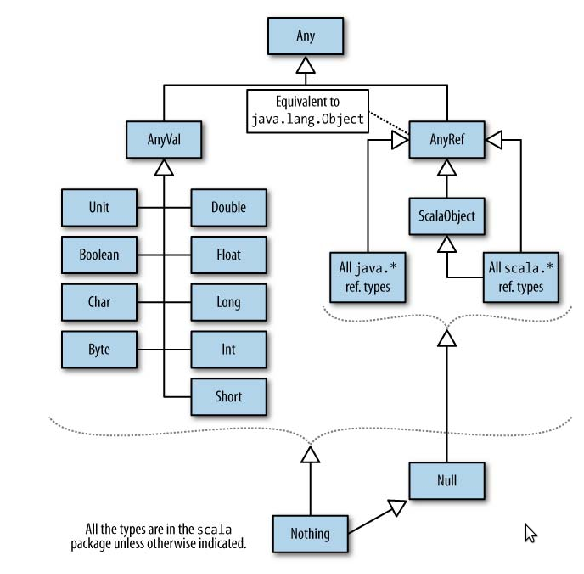
\includegraphics[scale=0.7]{bilder/typhierarchie.png}
\end{center}
\end{figure}


\begin{itemize}
  \item alle \texttt{AnyVal} Instanzen sind immutable \und 
  alle \texttt{Anyvalue} Typen sind \textit{abstract final}
\end{itemize}


\subsection{Linearisierung der Objekthierarchie}
betrachte folgendes Beispiel:

\lstinputlisting[label=src:linearization_object_hierarchiy.scala]{beispiele/linearization_object_hierarchiy.scala}


hier ist der Linearisierungsalso, den Scala verwendet:

\begin{enumerate}
  \item Put the actual type of the instance as the first element.
  \item Starting with the rightmost parent type and working left, compute the linearization
of each type, appending its linearization to the cumulative linearization. (Ignore
ScalaObject, AnyRef, and Any for now.)
  \item Working from left to right, remove any type if it appears again to the right of the
current position.
  \item Append ScalaObject, AnyRef, and Any.
\end{enumerate}
\pagebreak


\section{FP in Scala}


\subsection{Was FP ist}
\begin{itemize}
  \item haben keine Seiteneffekte, d.h. Analyse, Testen \und debuggen
  werden leichter
  \item \textit{referential transparency}, d.h. man kann eine Funktion
  in jeden beliebigen Kontext aufrufen \und muss keine Sorgen um den
  Kontext machen in dem die Funktion aufgerufen wird
  \item in FP sind Variablen immutable
\end{itemize}


\subsection{FP in Scala}
\begin{itemize}
  \item \ulab{Merke}: eine Funktion, die \texttt{Unit} zurückgibt,
  hat pure Seiteneffekte, denn ansonsten ist die Funktion sinnlos,
  da sie ja nichts zurückgibt
  
  \lstinputlisting[label=src:fp_list_map.scala]{beispiele/fp_list_map.scala}
  
  man kann die anonyme Funktion auch auf ein val drücken.
  
  \lstinputlisting[label=src:fp_list_map_value.scala]{beispiele/fp_list_map_value.scala}
  
  $\Rightarrow$ Faktor ist kein formaler Parameter sondern eine
  Referenz zu einer Variable in einen bstimmten scope, d.h. 
  der Compiler kreiert ein \textit{closure}
\end{itemize}


\subsection{Rekursion}
\begin{itemize}
  \item verhindert mutable Variablen
  \item aber Performanz-Overheadn \und Risiko des Stackoverflows
  \item Performaz-Prosb können mit \textit{memorization} \und 
  Stackoverflows können durch Umwandlung in eine spezielle 
  Schleife (Tail Calls \und Tail-Call Optimierung) verbessert
  werden
\end{itemize}


\subsection{Tail Calls und Tail-Call Optimierung}
\begin{itemize}
  \item Tail Call, d.h. wenn eine Funktion sich erst bei ihren
  finalen Durchlauf selbst aufruft $\Rightarrow$ es ist die leichteste
  Art der Rekursion, die man in eine normale Schleife umwandeln kann
  \item Schleifen verhindern die Gefahr eines Stackoverflows
  
  \lstinputlisting[label=src:factorial_recursive_and_tail_call.scala]{beispiele/factorial_recursive_and_tail_call.scala}
\end{itemize}


\subsection{Funktionale Datenstrukturen}
\begin{itemize}
  \item \textbf{Listen}: tauchen ganz oft in FP auf
  
  \lstinputlisting[label=src:lists_fp.scala]{beispiele/lists_fp.scala}
  
  \item \textbf{hash/dictionary/map}
    
  \item \textbf{Mengen}: sind wie Listen, aber ihnen kann jedes
  Element nur einmal vorkommen; Element Iteration geht in O(n)
\end{itemize}


\subsection{Traversieren, Mapping, Filtering, Folding und Reducing}
\begin{itemize}
  \item traveriseren geht mit der \texttt{foreach}:
  
  \lstinputlisting[label=src:foreach.scala]{beispiele/foreach.scala}
  
  \item \texttt{map}: wandelt eine Collection in eine neue Collection um,
  in der die Anzahl der Elemente gleich der Anzahl der Ursprungscollection
  ist
  
  \lstinputlisting[label=src:map.scala]{beispiele/map.scala}
  
  \item \texttt{filter} wird verwendet, um beim Traversieren durch eine
  Collection bestimmte Elemente herauszufiltern:
  
  \lstinputlisting[label=src:filter.scala]{beispiele/filter.scala}
  
  \item \texttt{folding} \und \texttt{reducing} werden beide verwendet, um
  eine collection zu schrumpfen, wobei folding immer mit einem 
  \textit{seed} beginnt:
  
  \lstinputlisting[label=src:folding_reducing.scala]{beispiele/folding_reducing.scala}  
\end{itemize}


\subsection{Pattern Matching}
\begin{itemize}
  \item ist das für FP, was Kapselung für OOP ist
  \item Pattern Matching ist ein eleganter Weg, um Objekte so zu zerlegen,
  dass sie in der erforderliche Verarbeitung passen
\end{itemize}


\subsection{Partielle Funktionen}
\begin{itemize}
  \item wenn an eine Funktion ein Unterstrich übergeben wird, dann handelt
  es sich um eine partielle Funktionen
  \item partielle Funktionen sind Aurücke, in denen nicht alle Argumente 
  einer Funktion auch von der Funktion übernommen werden
  
  \lstinputlisting[label=src:partial_functions_easy.scala]{beispiele/partial_functions_easy.scala}  
\end{itemize}


\subsection{Currying}
\begin{itemize}
  \item stammt vom Mathematiker Haskell Curry \und transformiert eine Funktion, die mehrere Parameter nimmt in eine Kettenfunktion, die nur einen
  Parameter nimmt
  \item in Scala werdem curried Funktion mit mehreren Parameterlisten
  definiert:
  
  \lstinputlisting[label=src:curried_functions.scala]{beispiele/curried_functions.scala}
  
  \item \ulab{Frage}: Wann verwendets man? Wenn man eine spezialisierte
  Funktion hat, die nur für bestimmte Daten geignet ist
\end{itemize}


\subsection{Implicits}
\begin{itemize}
  \item es kann manchmal vorkommen, dass man eine Instanz eines Typs hat 
  \und man diesen Typ in einen Kontext einsetzen möchte, in den es einen
  anderen aber vielleicht ähnlichen Typ geht
  
  $\Rightarrow$ Schlüsselwort \texttt{implizit} verwenden
  
  \lstinputlisting[label=src:implicit.scala]{beispiele/implicit.scala}  
\end{itemize}


\subsection{Lazy Vals}
\begin{itemize}
  \item das Schlüsselwort \texttt{lazy} benutzen:
  
  \lstinputlisting[label=src:lazy_vals.scala]{beispiele/lazy_vals.scala} 
  \item wenn man eine Variable als lazy deklariert, dann sollte man auch alle
  Verwendungen davon ebenfalls auf \textit{lazy} stellen 
\end{itemize}
\pagebreak


\section{Scala Typsystem}
\begin{itemize}
  \item Scala ist eine statisch typisierte Sprache \und das Typsystem ist 
  hier am fortschrittlichsten von allen Progsprachen, da es FP \und 
  OOP Benefits vereint
\end{itemize}


\subsection{Parametriesierte Typen}
\begin{itemize}
  \item bla
\end{itemize}


\subsection{Typen Bounds}
\begin{itemize}
  \item \texttt{A $<:$ AnyRef} means any type \texttt{A} that is a subtype of \texttt{AnyRef}
  \item bla, wurde an anderer Stelle besser erklärt
\end{itemize}


\subsection{Nothing und Null}
\begin{itemize}
  \item \texttt{Null} ist \texttt{final trait} \und kann nur eine Instanz haben
  \item \texttt{Nothing} ist \texttt{final trait} \und hat keine Instanz
\end{itemize}


\section{Fragen}
\begin{enumerate}
  \item Was sind \textbf{traits}?
  \begin{itemize}
    \item Ist eine besondere Variante eines \itbf{mixins}\footnote{zusammengehöriges, mehrfach verwendbares Bündel von Funktionalität bezeichnet, das zu einer Klasse hinzugefügt werden kann}. Ein Trait besitzt 
    eine gemeinsame Basisklasse mit der Klasse, auf die das Trait 
    angewendet wird.
  \end{itemize}
  \item Was ist der Unterschied zwischen val \und var?
  \begin{itemize}
    \item Variablen können in Scala jeweils den Wert 
    \textit{assign-once} \oder \textit{asign-many} haben
    \item \textit{assign-once}: mit \texttt{val} (ähnlich final
    in Java)
    \item \textit{assign-many}: mit \texttt{var}
    
    $\Rightarrow$ am besten immer val verwenden, denn je weniger
    sich Dinge $\Delta$ können, desto weniger Fehler können sich
    in den Code schleichen
  \end{itemize}
  \item Was drückt der folgende Ausdruck aus: $type S <: Subject$? Also was
  macht das $<:$?
  \item \textit{subclassing} bei mixins?
  \item \textbf{case-Klassen} generieren automatisch \textit{factory method} 
  mit denselben Argumenten als Primärkonstruktor
  \item Was sind \itbf{Views}\footnote{\textit{implicit conversions between
  types}; sie werden typischerweise angelegt, um neue Funktionalitäten
  für einen davorexistierenden Typ zu ergänzen}? Was ist im selben Zusammehang der 
  \textbf{implizit} Parameter\footnote{Argumente hierfür können bei einem
  Methodenaufruf weggelassen werden}?
  \item Was versteht man unter kontravariante Parametertypen?
\end{enumerate}



\subsection{Temproräres für DA}


\subsubsection{Statische versus Dynamsich typisierte Sprachen}
\begin{itemize}
  \item Typing $=_{df}$ \textit{A type system is a tractable syntactic method for preserving the absence of certain
program behaviors by classifying phrases according to the kinds of values they
compute.}

  \item ein Typsystem erlaubt es dem System zu sagen, was alles nicht
  stattfinden soll
  \item ein Typsystem kann verschiedene Fehler abfangen: \textit{like unsupported
operations on particular data structures, attempting to combine data in an undefined
way (e.g., trying to add an integer to a string), breaking abstractions, etc.
}
  \item in \itbf{statischer Typisierung} ist die Variable für seine gesamte Lebenszeit an einen Typ gebunden \und kann diesen nicht ändern
  \item in \itbf{dynamischer Typisierung} ist der Typ zum Wert \und 
  nicht zur Variable gebunden $\Rightarrow$ \textit{duck typung}; es wird
  deswegen von dynamik gesprochen, da der Typ einer Variable erst dann
  ausgewertet wird, wenn es zur Laufzeit verwendet wird
  \item Scala ist eine statisch typisierte Sprache
\end{itemize}


\subsubsection{Typinferenz}
\begin{itemize}
  \item darunter versteht man, dass man den Typ einer Variable schon anhand
  des Kontextest bestimmen kann (\uline{z.B.} \texttt{x = 1+ 3} $\Rightarrow$ 
  Compiler denkt sich also, dass \texttt{x} Integer ist)
\end{itemize}


% %%%%%%%%%%%%%%%%%%%%%%%%%%%%%%%%%%%%%%%%%
%       __       __  .___________.
%     |  |     |  | |           |
%    |  |     |  | `---|  |----`
%   |  |     |  |     |  |     
%  |  `----.|  |     |  |     
% |_______||__|     |__|     
%
% Literatur
% \end{comment}
\begin{comment}
\addcontentsline{toc}{section}{Literatur}
\bibliographystyle{acm}
\bibliography{literatur}
\end{comment}
\end{document}
